\section{Gigabit Ethernet}

1G/10G Ethernet IP contains PCS, PMA, Phy management and reset controller.

Transceiver: Combination tx/rx used when sending high-speed digital data/control signals acreoss physical Medium. Used in PHY layer of OSI model. Made up of the physical coding sublayer (PCS) and physical medium attachment (PMA). 

PCS: Digital logic that prepares and formats data for TX across a physical medium type or restores RX data to original form. Ex. Encoding, decoding, scrambling, descrambling.

PMA: Converts digital data to serial analog streams or reverse. 

\textbf{Data link Layer} Concerned with packaging data into frames and transmitting those frames on the network, performing error detection/correction and uniquely identifying network devices with an address(MAC) and flow control

MAC (Media Access Control):
\begin{itemize}
    \item Physical addressing: 48 bit address assigned to a device's network interface card (NIC)
    \item Logical topology: Logical network topologies
    \item Method of transmitting: CSMA/CD
\end{itemize}

LLC (Link Layer Control):

\begin{itemize}
\item Connection services: provides for acknowledgement of receipt of a message.
\begin{itemize}
    \item Flow control: Limits amount of data sender can send at one time 
    \item Error Control: Allows rx to let tx know when an expected data frame wasn't received or was corrupted by using a checksum.
\end{itemize}

\item Synchronizing transmissions
\end{itemize}

\subsection{1G/2.5G Ethernet IP}
In computer networking, Gigabit Ethernet (GbE or 1 GigE) is the term applied to transmitting Ethernet frames at a rate of a gigabit per second (1 billion bits per second) and is defined by the IEEE 802.3ab standard. There are five physical layer standards for Gigabit Ethernet using optical fiber (1000BASE\textendash X), twisted pair cable (1000BASE\textendash T), or shielded balanced copper cable (1000BASE\textendash CX). The IEEE 802.3z standard includes 1000BASE\textendash SX for transmission over multi\textendash mode fiber, 1000BASE\textendash LX for transmission over single\textendash mode fiber, and the nearly obsolete 1000BASE\textendash CX for transmission over shielded balanced copper cabling. These standards use 8b/10b encoding, which inflates the line rate by 25\%, from 1000 Mbit/s to 1250 Mbit/s, to ensure a DC balanced signal. The symbols are then sent using NRZ. Optical fiber transceivers are most often implemented as user\textendash swappable modules in SFP form or GBIC on older devices. IEEE 802.3ab, which defines the widely used 1000BASE\textendash T interface type, uses a different encoding scheme in order to keep the symbol rate as low as possible, allowing transmission over twisted pair. 
\begin{figure}[H]
\begin{center}
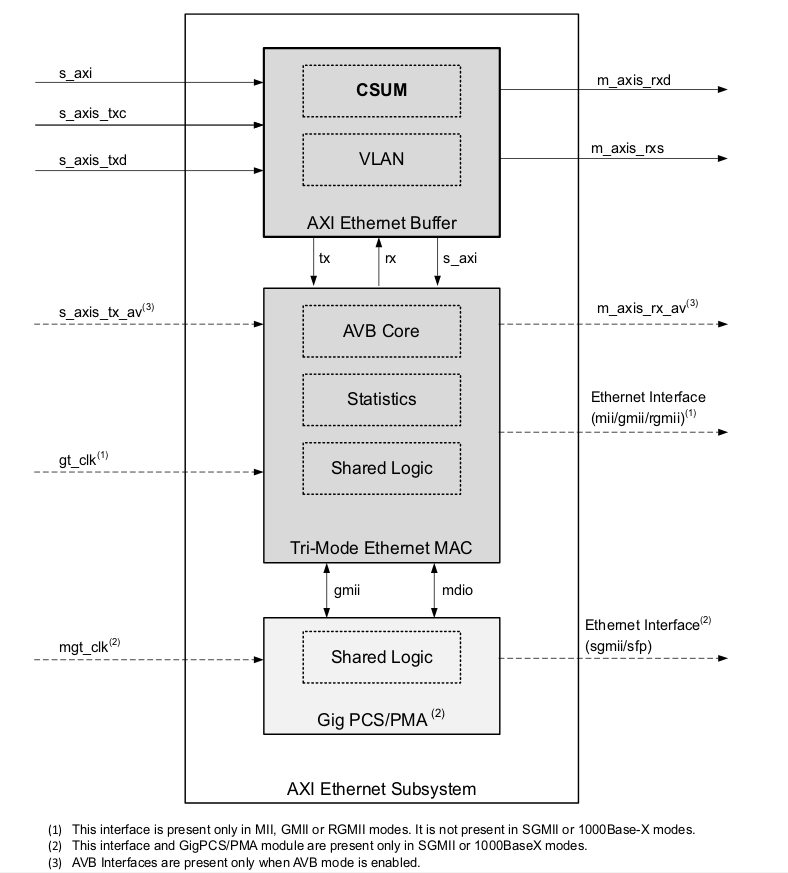
\includegraphics[width=\textwidth]{images/1G.png}
\caption{Internal block diagram of 1G/2.5G Ethernet Subsystem IP}
\label{1G}
\end{center}
\end{figure}
The AXI Ethernet Subsystem provides a control interface to internal registers via a 32\textendash bit AXI4\textendash Lite Interface subset. This AXI4\textendash Lite slave interface supports single beat read and write data transfers (no burst transfers). The transmit and receive data interface is via the AXI4\textendash Stream interface. This core has been designed incorporating the applicable features described in IEEE Std. 802.3\textendash 2012. This core supports the use of MII, GMII, SGMII, RGMII, and 1000BASE\textendash X interfaces to connect a media access control (MAC) to a physical\textendash side interface (PHY) chip. The internals of 1G/2.5G Ethernet Subsystem IP is shown in \figref{1G}.

The subsystem provides an AXI4\textendash Lite bus interface for a simple connection to the processor core to allow access to the registers. This AXI4\textendash Lite slave interface supports single beat read and write data transfers (no burst transfers). 32\textendash bit AXI4\textendash Stream buses are provided for moving transmit and receive Ethernet data to and from the subsystem. These buses are designed to be used with an AXI Direct Memory Access (DMA) IP core, AXI4\textendash Stream Data FIFO, or any other custom logic in any supported device. The AXI4\textendash Stream buses are designed to provide support for TCP/UDP partial or full checksum offload in hardware if required. 
The PHY side of the subsystem is connected to an off\textendash the\textendash shelf Ethernet PHY device, which performs the BASE\textendash T standard at 1 Gb/s, 100 Mb/s, and 10 Mb/s speeds. The PHY device can be connected using any of the following supported interfaces: GMII/MII, RGMII, or, by using the 1G/2.5G Ethernet PCS/PMA or SGMII module.


\subsection{10G/25G Ethernet IP}

\begin{figure}[H]
\begin{center}
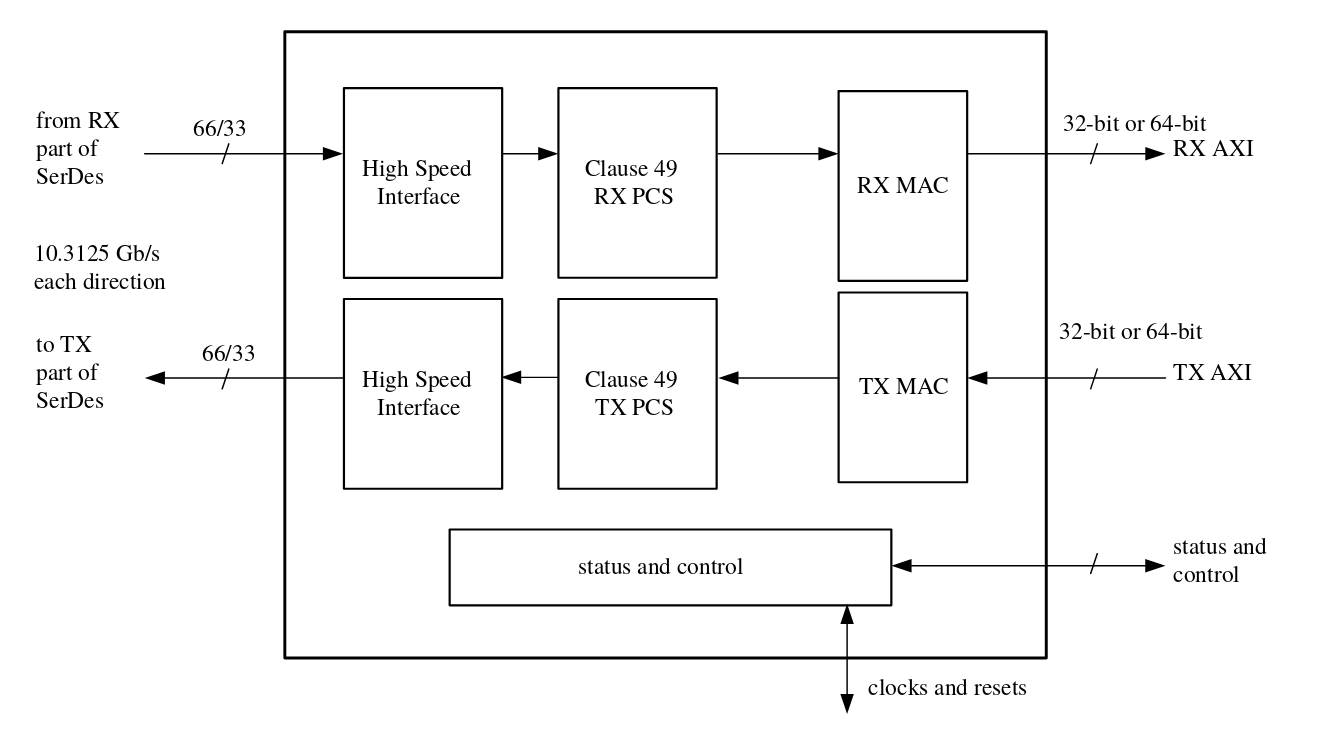
\includegraphics[width=\textwidth]{images/10G.png}
\caption{Internal block diagram of 10G/25G Ethernet Subsystem IP}
\label{10G}
\end{center}
\end{figure}

The Xilinx LogiCORE IP 10G/25G Ethernet solution provides a 10 Gigabit or 25 Gigabit per second (Gbps) Ethernet Media Access Controller integrated with a PCS/PMA in BASE\textendash R/KR modes or a standalone PCS/PMA in BASE\textendash R/KR modes. The core is designed to work with the latest Xilinx UltraScale and UltraScale+ FPGAs. The 25G Ethernet IP is designed to the new 25 Gb/s Ethernet Consortium standard and supports the demand of cloud data centers to enable lower cost and increased performance solutions between the server and the top of rack switch and to increase the front panel density by two. The internals of 10G/25G Ethernet Subsystem IP is shown in \figref{10G}.

\pagebreak
